\documentclass[11pt]{article}
\usepackage[margin=1in]{geometry}
\usepackage{booktabs}
\usepackage{graphicx}
\usepackage{hyperref}
\usepackage{enumitem}
\setlist{itemsep=2pt,topsep=4pt}
\newcommand{\code}[1]{\texttt{#1}}

\title{How often does a bounded check accept a wrong loop invariant?\\
\large CSE 216 project, Team 10: working summary and preliminary results}
\author{Working notes, 11 November 2026}
\date{}

\begin{document}
\maketitle

\noindent\fbox{\parbox{0.97\linewidth}{\small
\textbf{Status of this document.} These are working notes drafted with an AI assistant from the
experiment logs in the repository. The course policy does not allow AI-generated text in the
submitted report, so treat this as a source of facts, numbers and structure, and write the
report text yourselves. Every number here is produced by \code{src/analyze.py} from files in
\code{results/}.}}

\section{The question}

Small language models are being trained to write loop invariants for C programs. The training
signal comes from an automatic grader. A full software verifier is the most trustworthy grader,
but one check takes seconds to minutes, and a training run needs many thousands of checks. So
people use a cheaper grader: a bounded model checker that only explores the first $k$ iterations
of each loop.

A bounded check can accept an invariant that is false, because the violation may only show up
after more than $k$ iterations. Our question is how often that happens in practice:

\begin{quote}
Among loop invariants written by small language models, what share of the wrong ones does a
bounded check with bound $k$ accept, and how does that share change with $k$?
\end{quote}

We do no model training. We sample invariants, grade each one with both graders, and count
disagreements.

\section{Where the question comes from}

Loop-R1 (preprint) trains 1 to 2 billion parameter models with reinforcement learning to write
loop invariants. One term of its reward is bounded model checking with ESBMC at unwinding bound
$k<10$. In the limitations section the authors write that this ``may introduce false positives
by accepting invariants that hold only under bounded execution.'' The paper names the risk and,
in the parts we read, does not measure it. The code is not released.

Two neighbouring results already exist and we do not repeat them. Loop-R1 already reports that
reinforcement learning adds little on top of supervised fine-tuning for this task. Quokka
(InvBench) already reports that many accepted invariants only restate the assertion.

Our prior-work search for a measurement of bounded-versus-full disagreement on model-written
invariants was thin (Google Scholar, first page of results, plus the papers listed in
Section~\ref{sec:refs}). The honest wording is ``we found no prior measurement.''

\section{Background in four definitions}

\begin{description}[leftmargin=1.2em]
\item[Loop invariant.] A condition over program variables that holds every time execution reaches
the top of the loop body.
\item[Correctness query.] The program with \code{assert(candidate)} inserted at the top of the loop
body. The candidate is a true invariant exactly when this assertion can never fail.
\item[Full verifier.] UAutomizer (Ultimate Automizer, SV-COMP 2025 release). It answers TRUE (proved
for all executions), FALSE (a failing execution exists), or gives no answer (timeout or UNKNOWN).
\item[Bounded check.] ESBMC 8.6 with \code{--unwind k --no-unwinding-assertions}. It explores
executions with at most $k$ entries into each loop body and ignores longer ones. We measured this
on a toy loop: a violation on the $n$-th body entry is found exactly when $k \ge n$.
\end{description}

A bounded check that reports a violation has a concrete failing execution, so in principle it
never rejects a true invariant. Its only theoretical error is accepting a false one. That is the
soundness gap studied in the course under bounded model checking.

\section{Setup}

\begin{description}[leftmargin=1.2em]
\item[Programs.] The InvBench evaluation set as distributed with Wonda: 219 C programs with 362
loops, split by Wonda's rule into easy (239 loops) and hard (123 loops) according to how long
the verifier needs without help.
\item[Candidates, batch 1.] One invariant per loop from each of three untrained models
(Qwen3-0.6B, Qwen3-1.7B, Qwen3-4B-Instruct), 1{,}086 candidates, using Wonda's prompt and
sampling settings.
\item[Candidates, batch 2.] Eight invariants per loop from Wonda's published fine-tuned
4B model (\code{idopinto/Wonda-Qwen3-4B-Instruct-2507-V2-gt2-e2}), 2{,}896 candidates.
\item[Full grader.] UAutomizer on the correctness query, 30\,s limit on easy loops and 120\,s on
hard loops.
\item[Cheap grader.] ESBMC on the same query at $k \in \{1,2,5,10,20,50\}$, 30\,s limit, with
\code{--32 --no-pointer-check --no-bounds-check --no-div-by-zero-check --force-malloc-success}
so that only the inserted assertion counts.
\end{description}

A candidate counts as \emph{wrong} only when UAutomizer returns FALSE. Timeouts are kept as a
separate ``no answer'' category for both graders and are never counted as rejections.

\section{Preliminary results}
\label{sec:results}


All 3{,}982 sampled candidates were processed. 3{,}935 are syntactically valid and were graded
by both graders. UAutomizer proved 1{,}628 of them, found 2{,}016 wrong, and gave no answer on 291.

\subsection{How many wrong invariants does the bounded check accept?}

\begin{center}
\begin{tabular}{rrrrr}
\toprule
bound $k$ & accepted & accepted but wrong & 95\% CI & wrong that slip through \\
\midrule
1 & 2503 & 737 (29.4\%) & 27.7--31.3\% & 737/2016 (36.6\%) \\
2 & 1849 & 119 (6.4\%) & 5.4--7.6\% & 119/2016 (5.9\%) \\
5 & 1616 & 27 (1.7\%) & 1.2--2.4\% & 27/2016 (1.3\%) \\
10 & 1521 & 27 (1.8\%) & 1.2--2.6\% & 27/2016 (1.3\%) \\
20 & 1321 & 26 (2.0\%) & 1.3--2.9\% & 26/2016 (1.3\%) \\
50 & 994 & 10 (1.0\%) & 0.5--1.8\% & 10/2016 (0.5\%) \\
\bottomrule
\end{tabular}

\end{center}

\noindent ``Wrong that slip through'' has a fixed denominator, the 2{,}016 candidates UAutomizer
refuted. At $k=1$ more than a third of them are accepted. At $k=2$ about 6\%. From $k=5$ on it
is about 1\%. At the bound Loop-R1 describes ($k=10$) it is 27 of 2{,}016 (1.3\%, 95\% interval
0.9 to 1.9).

\begin{center}
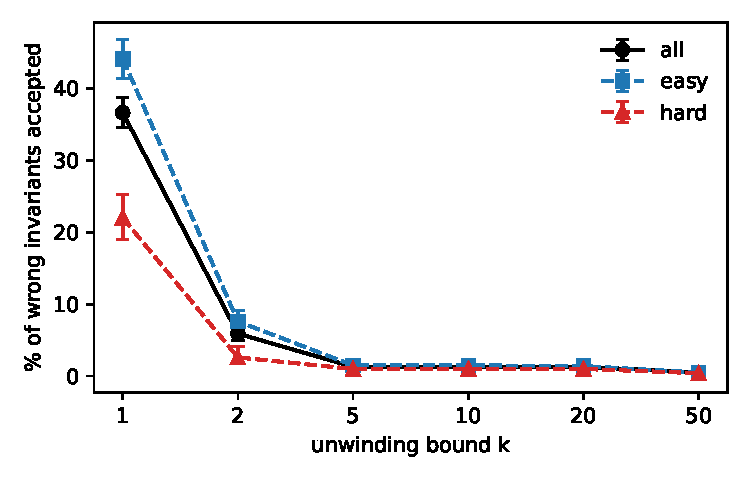
\includegraphics[width=0.6\linewidth]{../results/fig_bound_curve.pdf}
\end{center}

\subsection{Most of what remains at $k=10$ is not caused by the bound}

We read all 27 cases. They fall into two groups.

\begin{itemize}
\item \textbf{4 cases on one loop} (\code{nested\_delay\_notd2}) are true bound effects: ESBMC
accepts up to $k=20$ and rejects at $k=50$. Example candidate: \code{st == 0}.
\item \textbf{23 cases on six list-manipulating programs} are comparisons between a pointer and
zero, such as \code{0 < head}. UAutomizer refutes them; ESBMC accepts them at most bounds, including
$k=50$ where it finishes. A larger bound does not help, so this looks like a difference in how the two
tools model pointer ordering. We have not yet confirmed the cause.
\end{itemize}

Split by program type at $k=10$: on programs that do not allocate memory, 4 of 1{,}741 wrong
invariants are accepted (0.2\%, interval 0.1 to 0.6). On programs that do, 23 of 275 (8.4\%,
interval 5.6 to 12.2).

\subsection{The opposite disagreement}

34 candidates (20 distinct invariants on 10 loops) were proved by UAutomizer and rejected by
ESBMC with a concrete failing execution. All the ones we inspected involve signed arithmetic
that overflows, for example \code{a * b == x * y + z} with \code{int a, b} and
\code{long long x, y, z}. See Section~\ref{sec:learned}, item~2.

\subsection{A larger bound is not free}

Median time for one correctness check: UAutomizer 7.7\,s on easy loops and 7.4\,s on hard loops;
ESBMC at $k=10$ about 0.4\,s. UAutomizer gave no answer on 5.2\% of easy and 11.6\% of hard
candidates. The bounded check has its own failures, and they grow with the bound: among the
1{,}628 invariants UAutomizer proved, ESBMC hit its 30\,s limit on 1.8\% at $k=1$, 12.8\% at
$k=10$ and 41.7\% at $k=50$. So raising the bound trades fewer false accepts for more timeouts.

\subsection{Does the cheap grader pick good answers?}

Batch 2 has eight samples for each of the 362 loops. A pick is good if UAutomizer proves it.

\begin{center}
\begin{tabular}{lrl}
\toprule
rule for picking one sample per loop & good picks & 95\% interval \\
\midrule
first sample & 168/362 (46.4\%) & 41.3--51.6 \\
first sample accepted at $k=1$ & 210/362 (58.0\%) & 52.9--63.0 \\
first sample accepted at $k=2$ & 249/362 (68.8\%) & 63.8--73.3 \\
first sample accepted at $k=5$ & 255/362 (70.4\%) & 65.5--74.9 \\
first sample accepted at $k=10$ & 253/362 (69.9\%) & 65.0--74.4 \\
first sample accepted at $k=50$ & 238/362 (65.7\%) & 60.7--70.4 \\
best possible (any sample proved) & 277/362 (76.5\%) & 71.9--80.6 \\
\bottomrule
\end{tabular}
\end{center}

\noindent The bounded check at $k=5$ or $k=10$ recovers most of the gap between taking the
first sample and the best possible choice. $k=50$ is worse than $k=5$ because of timeouts.

\subsection{By split and by model}

At $k=10$ the slip-through count is 20 of 1{,}329 on easy loops and 7 of 687 on hard loops. By
batch it is 1 of 645 for the three untrained models and 26 of 1{,}371 for the fine-tuned 4B
model; the fine-tuned model is the one that writes the pointer comparisons. Per-model tables
are in \code{results/summary.md}.

\subsection{What this means for the question}

On this benchmark, the bound is a small source of error once $k \ge 5$ and a large one at
$k \le 2$. The disagreements that remain at $k=10$ come mostly from the two tools modelling C
differently (pointer ordering in one direction, integer overflow in the other). The benchmark
also favours the bounded check, because many of its loops are short; see Section~\ref{sec:limits}.


\section{Things we learned while building the cheap grader}\label{sec:learned}

These came from inspecting individual disagreements, and each one changed the numbers.

\begin{enumerate}
\item \textbf{Memory allocation.} ESBMC by default lets \code{malloc} return \code{NULL};
UAutomizer assumes it succeeds. Before we added \code{--force-malloc-success}, ESBMC rejected
invariants such as \code{x != NULL} that UAutomizer had proved. 60 of the 362 loops are in
programs that allocate memory.
\item \textbf{Signed integer overflow.} ESBMC models \code{int} as 32-bit values that wrap
around. UAutomizer proved some invariants that are false under wraparound. Example:
\code{(x > 0) || (y > 0) || (z > 0)} on \code{benchmark46\_disjunctive}, where ESBMC finds
\code{z = 2147483647} followed by \code{z++}. Re-running ESBMC with \code{--ir} (mathematical
integers) on three such cases made all three disagreements disappear. So these are two tools
answering slightly different questions, and the invariant's status depends on which integer
semantics is intended.
\item \textbf{Missing header.} The benchmark programs use \code{NULL} without including a header.
UAutomizer accepts that; ESBMC needs a one-line definition.
\end{enumerate}

Item 2 is the more interesting one for the report: the ``full'' grader is itself only as good as
its model of the language.

\section{Limits of what we can claim}\label{sec:limits}

\begin{itemize}
\item \textbf{Our bounded check is a reconstruction.} Loop-R1's code is not public. We follow the
one-sentence description in the paper. Their reward also has an SMT inductiveness term and a
consistency term that we do not reproduce, so our numbers describe the bounded-check component
only, not their whole reward.
\item \textbf{The benchmark has many short loops.} 103 of the 362 loops are in programs whose
loops are capped by a small constant counter (file names containing \code{unwindbound}). A bounded
check is complete on those once $k$ reaches the cap. Results may differ on programs with long
running loops.
\item \textbf{No answer is common on hard loops.} Where UAutomizer times out we cannot say whether
a cheap accept is right or wrong. The tables report this share separately.
\item \textbf{Timing under load.} Both graders ran concurrently on one 32-core machine, which
slows individual checks and may turn some slow answers into timeouts.
\item \textbf{Four models from one family and one fine-tuned checkpoint.} All are Qwen3 based.
\end{itemize}

\section{Plan to the report}

\begin{enumerate}
\item Week of Nov 11: finish both graders on batch 2, add the sufficiency query so each candidate
gets Wonda's 0 to 3 grade, add a second ESBMC mode with mathematical integers.
\item Week of Nov 16: re-run timeouts with a longer limit on an idle machine; sample from
Wonda's fine-tuned 0.6B and 1.7B models; add a random-testing grader as a second cheap check.
\item Week of Nov 23: programs with long loops (remove or raise the built-in counter caps) to see
whether the low slip-through rate survives; write up examples.
\item Nov 30 to Dec 4: freeze results, slides. Dec 9 presentation, Dec 11 report.
\end{enumerate}

\section{Connection to the course}

The project is a measurement of the gap between bounded model checking and unbounded
verification on a concrete workload: the bounded check under-approximates the set of executions,
so an ``accept'' is not a proof. The second finding (integer semantics) is about the modelling
step that precedes any verification: two sound tools can disagree because they formalise the
program differently.

\section{Sources}
\label{sec:refs}

\begin{itemize}
\item Loop-R1 preprint: \url{https://www.ai2wj.com/data/Loop-R1-preprint.pdf}
\item Wonda: arXiv:2603.15510, code at \url{https://github.com/idopinto/wonda}
\item Quokka / InvBench: arXiv:2509.21629
\item ESBMC: \url{https://github.com/esbmc/esbmc} (v8.6)
\item Ultimate Automizer: SV-COMP 2025 release
\end{itemize}

\end{document}
